\documentclass[aps,pra,showpacs,amsmath,amssymb,nofootinbib,longbibliography,superscriptaddress
]{revtex4-1}

%\documentclass[a4paper]{quantumarticle}
%\newcommand{\onlinecite}{\cite}
%\pdfoutput=1
%\usepackage{mcite}
%\usepackage[sort&compress,numbers]{natbib}
%\bibliographystyle{apsrev4-1}


\usepackage[pdftex]{graphicx}
\usepackage[usenames,dvipsnames]{xcolor}
\usepackage{epstopdf}
\usepackage{tikz}    % Include the tikz package for drawing
\usepackage{mathtools}

\usepackage[normalem]{ulem}


\usepackage[utf8]{inputenc}
\usepackage[T1]{fontenc}

\usepackage{beramono}
\usepackage{listings}

\usepackage{lmodern}

\usepackage{amssymb,amsmath,amsthm}

\usepackage{bbm}

\usepackage{subcaption}

\usepackage{algorithm}
\usepackage{algpseudocode}

\usepackage{graphicx}
\usepackage{subcaption}


\usepackage{mathtools}
\DeclarePairedDelimiter\bra{\langle}{\rvert}
\DeclarePairedDelimiter\ket{\lvert}{\rangle}
\DeclarePairedDelimiterX\braket[2]{\langle}{\rangle}{#1\,\delimsize\vert\,\mathopen{}#2}


\usepackage[justification=raggedright,singlelinecheck=false]{caption}

\DeclareMathAlphabet{\mathbbmsl}{U}{bbm}{m}{sl}

\newtheorem{theorem}{Theorem}
\theoremstyle{definition}
\newtheorem{definition}{Definition}

\theoremstyle{remark}
\newtheorem*{remark}{Remark}

\newtheorem{corollary}{Corollary}[theorem]
\newtheorem{lemma}[theorem]{Lemma}
\renewcommand{\qedsymbol}{$\blacksquare$}

\renewcommand{\lstlistingname}{Code Block}

\newcommand{\patbox}[1]{\vspace{2mm}\noindent\fbox{\parbox{0.47\textwidth}{\hspace{1mm}\parbox{\columnwidth}{\hspace{1mm}\\#1\vspace{1.5mm}}}}\\}

\lstdefinelanguage{julia}%
  {morekeywords={abstract,break,case,catch,const,continue,do,else,elseif,%
      end,export,false,for,function,immutable,import,importall,if,in,%
      macro,module,otherwise,quote,return,switch,true,try,type,typealias,%
      using,while},%
   sensitive=true,%
   alsoother={\$},%
   morecomment=[l]\#,%
   morecomment=[n]{\#=}{=\#},%
   morestring=[s]{"}{"},%
   morestring=[m]{'}{'},%
     literate={é}{{\'e}}1
           {è}{{\`e}}1
           {ù}{{\`u}}1
}[keywords,comments,strings]%

\lstset{%
    language          = julia,
    basicstyle        = \ttfamily,
    keywordstyle      = \bfseries\color{blue},
    numbers           = left,
    numbers           = none,
    stringstyle       = \color{magenta},
    commentstyle      = \color{ForestGreen},
    showstringspaces  = false,
    frame             = single, 
    inputencoding     = latin1,
    breaklines        = true,
    breakatwhitespace = true
}

\newcommand{\FRrefsec}[1]{sec.~\ref{#1}}
\newcommand{\FRreffig}[1]{fig.~\ref{#1}}
\newcommand{\FRrefeq}[1]{eq.~\ref{#1}}

\newcommand{\ENrefsec}[1]{Sec.~\ref{#1}}
\newcommand{\ENreffig}[1]{Fig.~\ref{#1}}
\newcommand{\ENrefeq}[1]{Eq.~\ref{#1}}



\newcommand{\Ham}{\hat{\mathcal{H}}}
\newcommand{\Spin}{\hat{S}}
\newcommand{\A}{\hat{A}{}}
\newcommand{\B}{\hat{B}{}}
\newcommand{\M}{\hat{M}}
\newcommand{\densmat}{\hat{\rho}}
\newcommand{\U}{\hat{U}{}}
\newcommand{\D}{\hat{D}{}}
\newcommand{\V}{\hat{V}{}}
\newcommand{\X}{\hat{X}{}}
\newcommand{\W}{\hat{W}{}}
\newcommand{\bigOmega}{\hat{\Omega}{}}
\newcommand{\bigLambda}{\hat{\Lambda}{}}
\newcommand{\bigGamma}{\hat{\Gamma}{}}


\newcommand{\I}{\hat{I}}
\newcommand{\0}{\hat{0}}

\newcommand{\x}{\mathbf{x}}
\newcommand{\dx}{\mathrm{d}\mathbf{x}}

\newcommand{\Z}{\mathcal{Z}}

\newcommand{\dt}{\mathrm{d}t}









   \newenvironment{xabstract}
{\onecolumngrid
    \list{}{%
        \setlength{\leftmargin}{.5in}% 
        \setlength{\rightmargin}{\leftmargin}%
        }%
        \item\relax}
        {\endlist}




\usepackage[compat=1.1.0]{tikz-feynman}




%\usepackage{chngcntr}


\usepackage[hidelinks]{hyperref}


\begin{document}

\title{Maxwell-Bloch Equations for the Simulation of Squeezed Light Generation in an Optical Resonator}
\author{Aaron Dayton}
\date{\today}

\maketitle
\tableofcontents

\section{Hamiltonian Formulation}

\textcolor{red}{NOTE: THIS IS NOT THE MAIN DERIVATION - THE MAIN DERIVATION IS THE QUANTUM VERSION IN MBE.tex - DO NOT USE THIS FILE EXCEPT FOR SPARE PARTS AS IT DEVIATES FROM THE UPDATED AND CORRECTED DERIVATION STEPS - THIS IS CURRENTLY INCORRECT!!!}

The first step in Hamiltonian formulation is system definition. We are modelling a 4-level diamond system as depicted in Fig.~\ref{DiamondAtom}. For this system, the choice of the ground state energy is arbitrary, and all other energies can be defined in terms of their differences as $\omega_2 = \omega_1 + \omega_{12}$, $\omega_3 = \omega_1 + \omega_{13}$, and $\omega_4 = \omega_{2} + \omega_{24} = \omega_{3} + \omega_{34}$.

\begin{figure}[htbp]
  \centering
  \begin{subfigure}{0.45\textwidth}
    \centering
    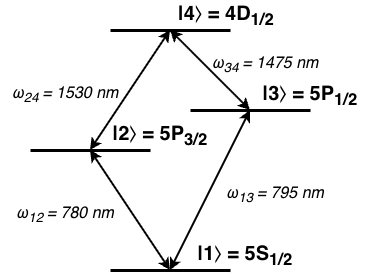
\includegraphics[width=\columnwidth]{Figs/DiamondAtom.png}
    \caption{A diamond configuration atomic system with  non-degenerate energy levels $\ket{1}, \ket{2}, \ket{3}, \ket{4}$ and respective energies $\hbar \omega_1$, $\hbar \omega_2$, $\hbar \omega_3$, and $\hbar \omega_4$. The system has allowed transitions $\ket{1} \leftrightarrow \ket{2}$, $\ket{1} \leftrightarrow \ket{3}$, $\ket{2} \leftrightarrow \ket{4}$, and $\ket{3} \leftrightarrow \ket{4}$}
    \label{DiamondAtom}
  \end{subfigure}
  \hfill
  \begin{subfigure}{0.45\textwidth}
    \centering
    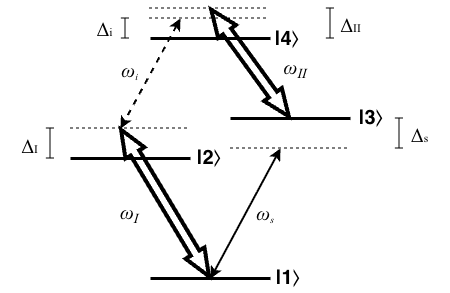
\includegraphics[width=\columnwidth]{Figs/DrivenDiamondAtom.png}
    \caption{A strong pump drives transition $\ket{1} \leftrightarrow \ket{2}$ at frequency $\omega_I$ with detuning $\Delta_I = \omega_I - \omega_{12}$, a separate strong pump drives transition $\ket{3} \leftrightarrow \ket{4}$ with detuning $\Delta_{II} = \omega_{II} - \omega_{34}$, a weak signal beam drives transition $\ket{1} \leftrightarrow \ket{3}$ with detuning $\Delta_{s} = \omega_{s} - \omega_{13}$, and a weak idler beam drives transition $\ket{2} \leftrightarrow \ket{4}$ with detuning $\Delta_{i} = \omega_{i} - \omega_{24}$.}
    \label{DrivenDiamondAtom}
  \end{subfigure}
  \caption{Diamond configuration atom diagrams.}
  \label{fig:twosidebyside}
\end{figure}

These states can be described without any interactions by the simple Hamiltonian

\begin{align}
    \hat{H}_0 &= \hbar \omega_1 \hat{\sigma}_{11} + \hbar \omega_2 \hat{\sigma}_{22} + \hbar \omega_3 \hat{\sigma}_{33} + \hbar \omega_4 \hat{\sigma}_{44}\\
    &= \hbar \left(\begin{array}{cccc}
        \omega_1 & 0 & 0 & 0\\
        0 & \omega_2 & 0 & 0\\
        0 & 0 & \omega_3 & 0\\
        0 & 0 & 0 & \omega_4\\
    \end{array}\right)
\end{align}


The reason we are attempting to obtain optical squeezing in the up-converted idler field is to transmit quantum information at telecom wavelengths. Therefore, we care about the quantized fields of the signal (input carrier of quantum information) and idler (output of frequency-converted quantum information) beams. Apply the theoretical resonant cavity approximation such that we consider photons in the Fock bases of the exact frequencies of the signal and idler beams to obtain the Hamiltonian

\begin{equation}
    \hat{H}_{photon} = \hbar \omega_{13} \hat{a}^{\dagger} \hat{a} + \hbar \omega_{24} \hat{b}^{\dagger} \hat{b}
\end{equation}

We then have the Hamiltonian describing these separate systems as


\begin{align}
    \hat{H}_S &= \hat{H}_0 + \hat{H}_{photon}\\
    &= \hbar \omega_1 \hat{\sigma}_{11} + \hbar \omega_2 \hat{\sigma}_{22} + \hbar \omega_3 \hat{\sigma}_{33} + \hbar \omega_4 \hat{\sigma}_{44}\nonumber \\
    &\;\;\;\;+ \hbar \omega_{13} \hat{a}^{\dagger} \hat{a} + \hbar \omega_{24} \hat{b}^{\dagger} \hat{b}
\end{align}


Each transition is driven by a laser as depicted in Fig.~\ref{DrivenDiamondAtom}. These driving fields cause significant coupling between states, requiring the definition of an interaction Hamiltonian. Under the dipole approximation following the procedure used in~\cite{QuantumInternet}, this interaction Hamiltonian takes the form  \textcolor{red}{NOTE - We do things slightly different than in the Du paper. They assume the dipole elements are all real-valued and swap $\sigma_{ij} \leftrightarrow \sigma_{ji}$ without swapping phases. This does not make any sense to me and seems like a hack or a mistake. We do not do this and end up with the addition of frequencies rather than detunings for the diagonal entries. I feel more confident with this because their method }

\subsection{Fully Semi-Classical Approach (Kupchak's Procedure)}


\begin{equation}
    \hat{H}_{Int} = - \hat{\mathbf{d}} \cdot \mathbf{E}
\end{equation}
\begin{equation}
    \hat{\mathbf{d}} = \vec{d}_{12} \hat{\sigma}_{12} + \vec{d}_{13} \hat{\sigma}_{13} + \vec{d}_{24} \hat{\sigma}_{24} + \vec{d}_{34} \hat{\sigma}_{34}
\end{equation}
\begin{equation}
    \mathbf{E} = \vec{E}_{I} + \vec{E}_{s} + \vec{E}_{i} + \vec{E}_{II}
\end{equation}
where $\mathbf{d}_{ij}$ is the dipole operator between states $i$ and $j$ and all fields are treated as strong semi-classical fields. We employ the slowly varying envelope approximation here such that each field can be separated into a rapidly oscillating component and a slowly-varying envelope $\varepsilon(t)$ as

\begin{align}
    \vec{E}_{I} &= \vec{\varepsilon}_I(t) e^{-i \omega_I t + i \vec{k}_I \cdot \vec{r}} + c.c.\\
    \vec{E}_{s} &= \vec{\varepsilon}_{s}(t) e^{-i \omega_s t + i \vec{k}_{s} \cdot \vec{r}} + h.c.\\
    \vec{E}_{i} &= \vec{\varepsilon}_{i}(t) e^{-i \omega_{i} t + i \vec{k}_{i} \cdot \vec{r}} + h.c.\\
    \vec{E}_{II} &= \vec{\varepsilon}_{II}(t) e^{-i \omega_{II} t + i \vec{k}_{II} \cdot \vec{r}} + c.c.\\
\end{align}
where $\hat{a}$ is the annihilation operator for the signal field, $\hat{b}$ is that of the idler field, $\vec{k}_j$ is the wavevector for each plane wave, and $\vec{r}$ is the position at which the field is experienced by the atom. This then gives
\begin{align}
    \hat{H}_{Int} = &\left(\vec{d}_{12} \cdot \vec{\varepsilon}_I(t) \hat{\sigma}_{12} e^{-i \omega_I t + i \vec{k}_I \cdot \vec{r}} + c.c.\right)\nonumber \\
    &+ \left(\vec{d}_{13} \cdot \vec{\varepsilon}_{s}(t) \hat{\sigma}_{13} e^{-i \omega_s t + i \vec{k}_{s} \cdot \vec{r}} + h.c.\right)\nonumber \\
    &+ \left(\vec{d}_{24} \cdot \vec{\varepsilon}_{i}(t) \hat{\sigma}_{24} e^{-i \omega_{i} t + i \vec{k}_{i} \cdot \vec{r}} + h.c.\right)\nonumber \\
    &+ \left(\vec{d}_{34} \cdot \vec{\varepsilon}_{II}(t) \hat{\sigma}_{34} e^{-i \omega_{II} t + i \vec{k}_{II} \cdot \vec{r}} + c.c.\right)
\end{align}
The Rabi frequency is the rate at which probability amplitudes between states oscillates in the presence of an electromagnetic field \cite{TODO} and is defined as

\begin{equation}
    \Omega = \frac{\vec{d} \cdot \vec{E}}{\hbar}
\end{equation}
so we have
\begin{align}
    \hat{H}_{Int} = &\left(\hbar \Omega_{I}(t) \hat{\sigma}_{12} e^{-i \omega_I t + i \vec{k}_I \cdot \vec{r}} + c.c.\right)\nonumber \\
    &+ \left(\hbar \Omega_{s}(t) \hat{\sigma}_{13} e^{-i \omega_s t + i \vec{k}_{s} \cdot \vec{r}} + h.c.\right)\nonumber \\
    &+ \left(\hbar \Omega_{i}(t) \hat{\sigma}_{24} e^{-i \omega_{i} t + i \vec{k}_{i} \cdot \vec{r}} + h.c.\right)\nonumber \\
    &+ \left(\hbar \Omega_{II}(t) \hat{\sigma}_{34} e^{-i \omega_{II} t + i \vec{k}_{II} \cdot \vec{r}} + c.c.\right)
\end{align}
where we can notice the utility of the slowly-varying envelop approximation as the Rabi oscillations change on the timescale of the envelope rather than the rapidly oscillating carrier field. This is analogous to the logic of the rotating wave approximation where the carrier field oscillates so rapidly that we can take its average effect on the dipole to be zero. This allows us to approximately separate the Rabi frequencies from the field frequencies in the above. \textcolor{red}{TODO - Check this line of reasoning with MacRae}.

Combining this with $\hat{H}_S$ we obtain a Hamiltonian coupling atomic states with the weak signal and idler fields as

\begin{align}
    \hat{H} &= \hat{H}_S + \hat{H}_{Int}\\
    &= \hbar \omega_1 \hat{\sigma}_{11} + \hbar \omega_2 \hat{\sigma}_{22} + \hbar \omega_3 \hat{\sigma}_{33} + \hbar \omega_4 \hat{\sigma}_{44}\nonumber \\
    &\;\;\;\;+ \hbar \omega_{13} \hat{a}^{\dagger} \hat{a} + \hbar \omega_{24} \hat{b}^{\dagger} \hat{b}\nonumber \\
    &\;\;\;\;+ \left(\hbar \Omega_{I}(t) \hat{\sigma}_{12} e^{-i \omega_I t + i \vec{k}_I \cdot \vec{r}} + c.c.\right)\nonumber \\
    &\;\;\;\;+ \left(\hbar \Omega_{s}(t) \hat{\sigma}_{13} e^{-i \omega_s t + i \vec{k}_{s} \cdot \vec{r}} + h.c.\right)\nonumber \\
    &\;\;\;\;+ \left(\hbar \Omega_{i}(t) \hat{\sigma}_{24} e^{-i \omega_{i} t + i \vec{k}_{i} \cdot \vec{r}} + h.c.\right)\nonumber \\
    &\;\;\;\;+ \left(\hbar \Omega_{II}(t) \hat{\sigma}_{34} e^{-i \omega_{II} t + i \vec{k}_{II} \cdot \vec{r}} + c.c.\right)
\end{align}

Then define the unitary transformation which rotates with state $\ket{1}$ as reference
\begin{align}
    \hat{U}_{atom} &= \hat{\sigma}_{11} + e^{i \omega_I t - i \vec{k}_I \cdot \vec{r}} \hat{\sigma}_{22} + e^{i \omega_s t - i \vec{k}_s \cdot \vec{r}} \hat{\sigma}_{33} + e^{i(\omega_{II} + \omega_s) t - i(\vec{k}_{II} + \vec{k}_s) \cdot \vec{r}} \hat{\sigma}_{44}
\end{align}
we then have the total unitary transformation of the coupled system as
\begin{equation}
    \hat{U} = \hat{U}_{atom} \otimes \hat{U}_{photon} = \left(\hat{\sigma}_{11} + e^{i \omega_I t - i \vec{k}_I \cdot \vec{r}} \hat{\sigma}_{22} + e^{i \omega_s t - i \vec{k}_s \cdot \vec{r}} \hat{\sigma}_{33} + e^{i(\omega_{II} + \omega_s) t - i(\vec{k}_{II} + \vec{k}_s) \cdot \vec{r}} \hat{\sigma}_{44}\right) \otimes e^{-i(\omega_s \hat{a}^{\dagger} \hat{a} + \omega_i \hat{b}^{\dagger} \hat{b})t}.
\end{equation}
The total Hamiltonian can then be unitarily transformed as

\begin{equation}
    \tilde{H} = \hat{U}^{\dagger} \hat{H} \hat{U} + i \hbar (\partial_t \hat{U}^{\dagger}) \hat{U}.
\end{equation}
First, compute the second term on the R.H.S.
\begin{equation}
    \hat{U}_{atom} = \left(\begin{array}{cccc}
        1 & 0 & 0 & 0\\
        0 & e^{i \omega_I t - i \vec{k}_I \cdot \vec{r}} & 0 & 0\\
        0 & 0 & e^{i \omega_s t - i \vec{k}_s \cdot \vec{r}} & 0\\
        0 & 0 & 0 & e^{i(\omega_{II} + \omega_s) t - i(\vec{k}_{II} + \vec{k}_s) \cdot \vec{r}}\\
    \end{array}\right)
\end{equation}
\begin{align}
    \partial_t \hat{U}_{atom}^{\dagger} &= \partial_t \left(\begin{array}{cccc}
        1 & 0 & 0 & 0\\
        0 & e^{-i \omega_I t + i \vec{k}_I \cdot \vec{r}} & 0 & 0\\
        0 & 0 & e^{-i \omega_s t + i \vec{k}_s \cdot \vec{r}} & 0\\
        0 & 0 & 0 & e^{-i(\omega_{II} + \omega_s) t + i(\vec{k}_{II} + \vec{k}_s) \cdot \vec{r}}\\
    \end{array}\right) \nonumber \\
    &=\left(\begin{array}{cccc}
        0 & 0 & 0 & 0\\
        0 & -i \omega_I U_{22}^{*} & 0 & 0\\
        0 & 0 & -i \omega_s U_{33}^{*} & 0\\
        0 & 0 & 0 & -i(\omega_{II} + \omega_s)U_{44}^{*}\\
    \end{array}\right) \nonumber
\end{align}
\begin{align}
    i \hbar (\partial_t \hat{U}_{atom}^{\dagger}) \hat{U}_{atom} &= i \hbar \left(\begin{array}{cccc}
        0 & 0 & 0 & 0\\
        0 & -i \omega_I U_{22}^{*} U_{22} & 0 & 0\\
        0 & 0 & -i \omega_s U_{33}^{*} U_{33} & 0\\
        0 & 0 & 0 & -i(\omega_{II} + \omega_s)U_{44}^{*} U_{44}\\
    \end{array}\right) \nonumber\\
    &= \hbar \left(\begin{array}{cccc}
        0 & 0 & 0 & 0\\
        0 & \omega_I & 0 & 0\\
        0 & 0 & \omega_s & 0\\
        0 & 0 & 0 & \omega_{II} + \omega_s
    \end{array}\right)\nonumber\\
    &= \hbar \omega_I \hat{\sigma}_{22} + \hbar \omega_s \hat{\sigma}_{33} + \hbar (\omega_{II} + \omega_s) \hat{\sigma}_{44}
\end{align}






Then computing the former term on the R.H.S we have
\begin{align}
    \hat{U}^{\dagger} \hat{H} \hat{U}
    &= \left(\hat{\sigma}_{11} + e^{-i \omega_I t + i \vec{k}_I \cdot \vec{r}} \hat{\sigma}_{22} + e^{-i \omega_s t + i \vec{k}_s \cdot \vec{r}} \hat{\sigma}_{33} + e^{-i(\omega_{II} + \omega_s) t + i(\vec{k}_{II} + \vec{k}_s) \cdot \vec{r}} \hat{\sigma}_{44}\right) \nonumber\\
    &\;\;\;\;\cdot\biggl[ \hbar \omega_1 \hat{\sigma}_{11} + \hbar \omega_2 \hat{\sigma}_{22} + \hbar \omega_3 \hat{\sigma}_{33} + \hbar \omega_4 \hat{\sigma}_{44}\nonumber \\
    &\;\;\;\;\;\;\;\;+ \hbar \left(\Omega_{I}(t) \hat{\sigma}_{12} e^{-i \omega_I t + i \vec{k}_I \cdot \vec{r}} + \Omega_{I}^*(t) \hat{\sigma}_{21} e^{i \omega_I t - i \vec{k}_I \cdot \vec{r}}\right)\nonumber \\
    &\;\;\;\;\;\;\;\;+ \hbar \left(\Omega_{s}(t) \hat{\sigma}_{13} e^{-i \omega_s t + i \vec{k}_{s} \cdot \vec{r}} + \Omega_{s}^*(t) \hat{\sigma}_{31} e^{i \omega_s t - i \vec{k}_{s} \cdot \vec{r}}\right)\nonumber \\
    &\;\;\;\;\;\;\;\;+ \hbar \left(\Omega_{i}(t) \hat{\sigma}_{24} e^{-i \omega_i t + i \vec{k}_{i} \cdot \vec{r}} + \Omega_{i}^*(t) \hat{\sigma}_{42} e^{i \omega_i t - i \vec{k}_{i} \cdot \vec{r}}\right)\nonumber \\
    &\;\;\;\;\;\;\;\;+ \hbar \left(\Omega_{II}(t) \hat{\sigma}_{34} e^{-i \omega_{II} t + i \vec{k}_{II} \cdot \vec{r}} + \Omega_{II}^*(t) \hat{\sigma}_{43} e^{i \omega_{II} t - i \vec{k}_{II} \cdot \vec{r}}\right)\biggr] \nonumber\\
    &\;\;\;\; \cdot \left(\hat{\sigma}_{11} + e^{i \omega_I t - i \vec{k}_I \cdot \vec{r}} \hat{\sigma}_{22} + e^{i \omega_s t - i \vec{k}_s \cdot \vec{r}} \hat{\sigma}_{33} + e^{i(\omega_{II} + \omega_s) t - i(\vec{k}_{II} + \vec{k}_s) \cdot \vec{r}} \hat{\sigma}_{44}\right)
\end{align}





Let us compute this using the facts that
\begin{equation}
    \hat{\sigma}_{ij} \hat{\sigma}_{kl} = \hat{\sigma}_{il} \delta_{jk},
\end{equation}
and
\begin{equation}
    \hat{\sigma}_{ij} \hat{\sigma}_{jk} \hat{\sigma}_{kl} = \hat{\sigma}_{il},
\end{equation}

\begin{align}
    \frac{\hat{U}^{\dagger} \hat{H} \hat{U}}{\hbar}
    &= \omega_1 \hat{\sigma}_{11} + \omega_2 \hat{\sigma}_{22} e^{-i \omega_I t + i \vec{k}_I \cdot \vec{r}} e^{i \omega_I t - i \vec{k}_I \cdot \vec{r}} \nonumber \\
    &\;\;\;\;+ \omega_3 \hat{\sigma}_{33} e^{-i \omega_s t + i \vec{k}_s \cdot \vec{r}} e^{i \omega_s t - i \vec{k}_s \cdot \vec{r}} + \omega_4 \hat{\sigma}_{44} e^{-i(\omega_{II} + \omega_s) t + i(\vec{k}_{II} + \vec{k}_s) \cdot \vec{r}} e^{i(\omega_{II} + \omega_s) t - i(\vec{k}_{II} + \vec{k}_s) \cdot \vec{r}} \nonumber \\
    &\;\;\;\;+ \left(\hat{\sigma}_{11} + e^{-i \omega_I t + i \vec{k}_I \cdot \vec{r}} \hat{\sigma}_{22} + e^{-i \omega_s t + i \vec{k}_s \cdot \vec{r}} \hat{\sigma}_{33} + e^{-i(\omega_{II} + \omega_s) t + i(\vec{k}_{II} + \vec{k}_s) \cdot \vec{r}} \hat{\sigma}_{44}\right) \nonumber\\
    &\;\;\;\;\cdot \biggl[ \left(\Omega_{I}(t) \hat{\sigma}_{12} e^{-i \omega_I t + i \vec{k}_I \cdot \vec{r}} + \Omega_{I}^*(t) \hat{\sigma}_{21} e^{i \omega_I t - i \vec{k}_I \cdot \vec{r}}\right)\nonumber \\
    &\;\;\;\;\;\;+ \left(\Omega_{s}(t) \hat{\sigma}_{13} e^{-i \omega_s t + i \vec{k}_{s} \cdot \vec{r}} + \Omega_{s}^*(t) \hat{\sigma}_{31} e^{i \omega_s t - i \vec{k}_{s} \cdot \vec{r}}\right)\nonumber \\
    &\;\;\;\;\;\;+ \left(\Omega_{i}(t) \hat{\sigma}_{24} e^{-i \omega_i t + i \vec{k}_{i} \cdot \vec{r}} + \Omega_{i}^*(t) \hat{\sigma}_{42} e^{i \omega_i t - i \vec{k}_{i} \cdot \vec{r}}\right)\nonumber \\
    &\;\;\;\;\;\;+ \left(\Omega_{II}(t) \hat{\sigma}_{34} e^{-i \omega_{II} t + i \vec{k}_{II} \cdot \vec{r}} + \Omega_{II}^*(t) \hat{\sigma}_{43} e^{i \omega_{II} t - i \vec{k}_{II} \cdot \vec{r}}\right)\biggr] \nonumber \\
    &\;\;\;\; \cdot \left(\hat{\sigma}_{11} + e^{i \omega_I t - i \vec{k}_I \cdot \vec{r}} \hat{\sigma}_{22} + e^{i \omega_s t - i \vec{k}_s \cdot \vec{r}} \hat{\sigma}_{33} + e^{i(\omega_{II} + \omega_s) t - i(\vec{k}_{II} + \vec{k}_s) \cdot \vec{r}} \hat{\sigma}_{44}\right)\nonumber
\end{align}
\begin{align}
    &= \omega_1 \hat{\sigma}_{11} + \omega_2 \hat{\sigma}_{22} + \omega_3 \hat{\sigma}_{33} + \omega_4 \hat{\sigma}_{44} \nonumber \\
    &\;\;\;\;+ \left(\hat{\sigma}_{11} + e^{-i \omega_I t + i \vec{k}_I \cdot \vec{r}} \hat{\sigma}_{22} + e^{-i \omega_s t + i \vec{k}_s \cdot \vec{r}} \hat{\sigma}_{33} + e^{-i(\omega_{II} + \omega_s) t + i(\vec{k}_{II} + \vec{k}_s) \cdot \vec{r}} \hat{\sigma}_{44}\right) \nonumber\\
    &\;\;\;\;\cdot \biggl[ \left(\Omega_{I}(t) \hat{\sigma}_{12} e^{-i \omega_I t + i \vec{k}_I \cdot \vec{r}} + \Omega_{I}^*(t) \hat{\sigma}_{21} e^{i \omega_I t - i \vec{k}_I \cdot \vec{r}}\right)\nonumber \\
    &\;\;\;\;\;\;+ \left(\Omega_{s}(t) \hat{\sigma}_{13} e^{-i \omega_s t + i \vec{k}_{s} \cdot \vec{r}} + \Omega_{s}^*(t) \hat{\sigma}_{31} e^{i \omega_s t - i \vec{k}_{s} \cdot \vec{r}}\right)\nonumber \\
    &\;\;\;\;\;\;+ \left(\Omega_{i}(t) \hat{\sigma}_{24} e^{-i \omega_i t + i \vec{k}_{i} \cdot \vec{r}} + \Omega_{i}^*(t) \hat{\sigma}_{42} e^{i \omega_i t - i \vec{k}_{i} \cdot \vec{r}}\right)\nonumber \\
    &\;\;\;\;\;\;+ \left(\Omega_{II}(t) \hat{\sigma}_{34} e^{-i \omega_{II} t + i \vec{k}_{II} \cdot \vec{r}} + \Omega_{II}^*(t) \hat{\sigma}_{43} e^{i \omega_{II} t - i \vec{k}_{II} \cdot \vec{r}}\right)\biggr] \nonumber \\
    &\;\;\;\; \cdot \left(\hat{\sigma}_{11} + e^{i \omega_I t - i \vec{k}_I \cdot \vec{r}} \hat{\sigma}_{22} + e^{i \omega_s t - i \vec{k}_s \cdot \vec{r}} \hat{\sigma}_{33} + e^{i(\omega_{II} + \omega_s) t - i(\vec{k}_{II} + \vec{k}_s) \cdot \vec{r}} \hat{\sigma}_{44}\right)
\end{align}
\begin{align}
    &= \omega_1 \hat{\sigma}_{11} + \omega_2 \hat{\sigma}_{22} + \omega_3 \hat{\sigma}_{33} + \omega_4 \hat{\sigma}_{44} \nonumber \\
    &\;\;\;\;+  \left(\Omega_{I}(t) \hat{\sigma}_{11} \hat{\sigma}_{12} \hat{\sigma}_{22} e^{i \omega_I t - i \vec{k}_I \cdot \vec{r}}  e^{-i \omega_I t + i \vec{k}_I \cdot \vec{r}} + \Omega_{I}^*(t) e^{-i \omega_I t + i \vec{k}_I \cdot \vec{r}} \hat{\sigma}_{22} \hat{\sigma}_{21} \hat{\sigma}_{11} e^{i \omega_I t - i \vec{k}_I \cdot \vec{r}}\right)\nonumber \\
    &\;\;\;\;+ \left(\Omega_{s}(t) \hat{\sigma}_{11} \hat{\sigma}_{13} \hat{\sigma}_{33} e^{i \omega_s t - i \vec{k}_s \cdot \vec{r}} e^{-i \omega_s t + i \vec{k}_{s} \cdot \vec{r}} + \Omega_{s}^*(t) e^{-i \omega_s t + i \vec{k}_s \cdot \vec{r}} \hat{\sigma}_{33} \hat{\sigma}_{31} \hat{\sigma}_{11} e^{i \omega_s t - i \vec{k}_{s} \cdot \vec{r}}\right)\nonumber \\
    &\;\;\;\;+ \Bigl(\Omega_{i}(t) e^{-i \omega_I t + i \vec{k}_I \cdot \vec{r}} \hat{\sigma}_{22} \hat{\sigma}_{24} \hat{\sigma}_{44} e^{i(\omega_{II} + \omega_s) t - i(\vec{k}_{II} + \vec{k}_s) \cdot \vec{r}} e^{-i \omega_i t + i \vec{k}_{i} \cdot \vec{r}} \nonumber \\
    &\;\;\;\;\;\;+ \Omega_{i}^*(t) e^{-i(\omega_{II} + \omega_s) t + i(\vec{k}_{II} + \vec{k}_s) \cdot \vec{r}} \hat{\sigma}_{44} \hat{\sigma}_{42} \hat{\sigma}_{22} e^{i \omega_I t - i \vec{k}_I \cdot \vec{r}} e^{i \omega_i t - i \vec{k}_{i} \cdot \vec{r}}\Bigr)\nonumber \\
    &\;\;\;\;+ \Bigl(\Omega_{II}(t) e^{-i \omega_s t + i \vec{k}_s \cdot \vec{r}} \hat{\sigma}_{33} \hat{\sigma}_{34} \hat{\sigma}_{44} e^{i(\omega_{II} + \omega_s) t - i(\vec{k}_{II} + \vec{k}_s) \cdot \vec{r}} e^{-i \omega_{II} t + i \vec{k}_{II} \cdot \vec{r}} \nonumber \\
    &\;\;\;\;\;\;+ \Omega_{II}^*(t) e^{-i(\omega_{II} + \omega_s) t + i(\vec{k}_{II} + \vec{k}_s) \cdot \vec{r}} \hat{\sigma}_{44} \hat{\sigma}_{43} \hat{\sigma}_{33} e^{i \omega_s t - i \vec{k}_s \cdot \vec{r}} e^{i \omega_{II} t - i \vec{k}_{II} \cdot \vec{r}}\Bigr) \nonumber \\ \nonumber \\
    &= \omega_1 \hat{\sigma}_{11} + \omega_2 \hat{\sigma}_{22} + \omega_3 \hat{\sigma}_{33} + \omega_4 \hat{\sigma}_{44} \nonumber \\
    &\;\;\;\;+ \left(\Omega_{I}(t) \hat{\sigma}_{12} + \Omega_{I}^*(t) \hat{\sigma}_{21} \right)\nonumber \\
    &\;\;\;\;+ \left(\Omega_{s}(t) \hat{\sigma}_{13} + \Omega_{s}^*(t) \hat{\sigma}_{31} \right)\nonumber \\
    &\;\;\;\;+ (\Omega_{i}(t) e^{i(\omega_{II} + \omega_s - \omega_I - \omega_i) t - i(\vec{k}_{II} + \vec{k}_s - \vec{k}_I - \vec{k}_{i}) \cdot \vec{r}} \hat{\sigma}_{24} + \Omega_{i}^*(t) e^{-i(\omega_{II} + \omega_s - \omega_I - \omega_i) t + i(\vec{k}_{II} + \vec{k}_s - \vec{k}_I - \vec{k}_{i}) \cdot \vec{r}} \hat{\sigma}_{42} )\nonumber \\
    &\;\;\;\;+ (\Omega_{II}(t) \hat{\sigma}_{34} + \Omega_{II}^*(t) \hat{\sigma}_{43} )
\end{align}
We can then impose the energy conservation condition and phase match condition (in that order as follows)
\begin{align}
    \omega_I + \omega_i &= \omega_s + \omega_{II}\\
    k_I + k_i &= k_s + k_{II}
\end{align}

\begin{align}
    \hat{U}^{\dagger} \hat{H} \hat{U}
    &= \hbar \Bigl(\omega_1 \hat{\sigma}_{11} + \omega_2 \hat{\sigma}_{22} + \omega_3 \hat{\sigma}_{33} + \omega_4 \hat{\sigma}_{44} \nonumber \\
    &\;\;\;\;\;\;+ \left(\Omega_{I}(t) \hat{\sigma}_{12} + \Omega_{I}^*(t) \hat{\sigma}_{21} \right)\nonumber \\
    &\;\;\;\;\;\;+ \left(\Omega_{s}(t) \hat{\sigma}_{13} + \Omega_{s}^*(t) \hat{\sigma}_{31} \right)\nonumber \\
    &\;\;\;\;\;\;+ (\Omega_{i}(t) \hat{\sigma}_{24} + \Omega_{i}^*(t) \hat{\sigma}_{42} )\nonumber \\
    &\;\;\;\;\;\;+ (\Omega_{II}(t) \hat{\sigma}_{34} + \Omega_{II}^*(t) \hat{\sigma}_{43} )\Bigr)
\end{align}
Thus we have
\begin{align}
    \tilde{H} &= \hat{U}^{\dagger} \hat{H} \hat{U} + i \hbar (\partial_t \hat{U}^{\dagger}) \hat{U} \nonumber \\
    &= \hbar \biggl(\omega_1 \hat{\sigma}_{11} + \omega_2 \hat{\sigma}_{22} + \omega_3 \hat{\sigma}_{33} + \omega_4 \hat{\sigma}_{44} \nonumber \\
    &\;\;\;\;\;\;+ \left(\Omega_{I}(t) \hat{\sigma}_{12} + \Omega_{I}^*(t) \hat{\sigma}_{21} \right)\nonumber \\
    &\;\;\;\;\;\;+ \left(\Omega_{s}(t) \hat{\sigma}_{13} + \Omega_{s}^*(t) \hat{\sigma}_{31} \right) \nonumber \\
    &\;\;\;\;\;\;+ ( \Omega_{i}(t) \hat{\sigma}_{24} + \Omega_{i}^*(t) \hat{\sigma}_{42} ) \nonumber \\
    &\;\;\;\;\;\;+ (\Omega_{II}(t) \hat{\sigma}_{34} + \Omega_{II}^*(t) \hat{\sigma}_{43} )\biggr)\nonumber \\
    &\;\;\;\;+ \hbar \biggl(\omega_I \hat{\sigma}_{22} + \omega_s \hat{\sigma}_{33} + (\omega_{II} + \omega_s) \hat{\sigma}_{44} \biggr) \nonumber \\
    &= \hbar \biggl(\omega_1 \hat{\sigma}_{11} + (\omega_2 + \omega_I) \hat{\sigma}_{22} + (\omega_3 + \omega_s) \hat{\sigma}_{33} + (\omega_4 + \omega_{II} + \omega_s) \hat{\sigma}_{44} \nonumber \\
    &\;\;\;\;\;\;+ \left(\Omega_{I}(t) \hat{\sigma}_{12} + \Omega_{I}^*(t) \hat{\sigma}_{21} \right)\nonumber \\
    &\;\;\;\;\;\;+ \left(\Omega_{s}(t) \hat{\sigma}_{13} + \Omega_{s}^*(t) \hat{\sigma}_{31} \right) \nonumber \\
    &\;\;\;\;\;\;+ (\Omega_{i}(t) \hat{\sigma}_{24} + \Omega_{i}^*(t) \hat{\sigma}_{42} ) \nonumber \\
    &\;\;\;\;\;\;+ (\Omega_{II}(t) \hat{\sigma}_{34} + \Omega_{II}^*(t) \hat{\sigma}_{43} )\biggr)\nonumber
\end{align}

We can then choose to arbitrarily shift the Hamiltonian by
\begin{align}
    \tilde{H} &\rightarrow \tilde{H} - \hbar \omega_1 \hat{\mathbbm{1}} \nonumber \\
    &\rightarrow \hbar \biggl[(\omega_2 - \omega_1 + \omega_I) \hat{\sigma}_{22} + (\omega_3 - \omega_1 + \omega_s) \hat{\sigma}_{33} + (\omega_4 - \omega_1 + \omega_{II} + \omega_s) \hat{\sigma}_{44} \nonumber \\
    &\;\;\;\;+ \left(\Omega_{I}(t) \hat{\sigma}_{12} + \Omega_{I}^*(t) \hat{\sigma}_{21} \right)+ \left(\Omega_{s}(t) \hat{\sigma}_{13} + \Omega_{s}^*(t) \hat{\sigma}_{31} \right) + ( \Omega_{i}(t) \hat{\sigma}_{24} + \Omega_{i}^*(t) \hat{\sigma}_{42} ) + (\Omega_{II}(t) \hat{\sigma}_{34} + \Omega_{II}^*(t) \hat{\sigma}_{43} ) \biggr] \nonumber
\end{align}
Apply the relations
\begin{align}
    &\omega_{12} = \omega_2 - \omega_1\\
    &\omega_{13} = \omega_3 - \omega_1\\
    &\omega_{24} = \omega_4 - \omega_2\\
    &\omega_{34} = \omega_4 - \omega_3\\
    &\Delta_a = \omega_{13} - \omega_s\\
    &\Delta_b = \omega_{24} - \omega_s
\end{align}
we have
\begin{align}
    \omega_{34} + \omega_{13} &= (\omega_4 - \omega_3) + (\omega_3 - \omega_1)\nonumber \\
    &= \omega_4 - \omega_1
\end{align}

\begin{align}
    \tilde{H} &= \hbar \biggl[(\omega_{12}+ \omega_I) \hat{\sigma}_{22} + (\omega_{13} + \omega_s) \hat{\sigma}_{33} + (\omega_{34} + \omega_{13} + \omega_{II} + \omega_s) \hat{\sigma}_{44} \nonumber \\
    &\;\;\;\;+ \left(\Omega_{I}(t) \hat{\sigma}_{12} + \Omega_{I}^*(t) \hat{\sigma}_{21} \right) + \left(\Omega_{s}(t) \hat{\sigma}_{13} + \Omega_{s}^*(t)\hat{\sigma}_{31} \right) + ( \Omega_{i}(t) \hat{\sigma}_{24} + \Omega_{i}^*(t) \hat{\sigma}_{42} ) + (\Omega_{II}(t) \hat{\sigma}_{34} + \Omega_{II}^*(t) \hat{\sigma}_{43} )\biggr]
\end{align}


\begin{align}
    \tilde{H} &= \hbar \left(\begin{array}{cccc}
        0 & \Omega_{I}(t) & \Omega_{s}(t) & 0\\
        \Omega_{I}^*(t) & \omega_{12} + \omega_I & 0 & \Omega_{i}(t) \\
        \Omega_{s}^*(t) & 0 & \omega_{13} + \omega_s & \Omega_{II}(t)\\
        0 & \Omega_{i}^*(t) & \Omega_{II}^*(t) & \omega_{34} + \omega_{13} + \omega_{II} + \omega_s\\
    \end{array}\right)
\end{align}






\bibliography{refs}


\end{document}